%!TEX TS-program = xelatex
\documentclass[a4paper, 12pt]{article}
\usepackage{barinovxesimple}
\geometry{top=25mm}
\geometry{bottom=35mm}
\geometry{left=35mm}
\geometry{right=20mm}
\setlist{labelindent=\parindent,leftmargin=*}
\begin{document}
\thispagestyle{empty}
\begin{center}
    \textit{Федеральное государственное автономное образовательное\\ учреждение высшего образования }

    \vspace{0.5ex}

        \textbf{«Московский физико-технический институт\\ (национальный исследовательский университет)»}
\end{center}

\vspace{10ex}

\begin{center}
    \vspace{13ex}

    \so{\textbf{Лабораторная работа №-.-.-}}

    \vspace{1ex}

    по курсу общей физики

    на тему:

    \textbf{\textit{<<>>}}

    \vspace{30ex}

    \begin{flushright}
        \noindent
        \textit{Работу выполнил:}\\  
        \textit{Баринов Леонид \\(группа Б02-827)}
    \end{flushright}
    \vfill
    Долгопрудный \\2019
\newpage
\setcounter{page}{1}
\fancyhead[R]{\nouppercase{\leftmark}}	
\end{center}

\section{Цель работы}
Исследовать излучение накаленных тел с различной испускательной
способностью, определить постоянные Планка и Стефана-Больцмана.

\section{Суть исследуемого явления}
Закон Стефана-Больцмана:
\begin{equation}
    W = \epsilon_\text{T} S \sigma T^4
    \label{eq:1}
\end{equation}
$W$ --- потребляемая нитью электрическая мощность. $S$ --- площадь
излучающей поверхности нити, $T$ --- температура нити, $\epsilon_T$
--- коэффициент серости, $\sigma$ --- постоянная Стефана-Больцмана. 


\section{Теория явления}
Абсолютное черное тело (АЧТ) --- тело, поглощающее все падающее на него
излучение. Энергия, излучаемая любым другим телом, может быть найдена
путем умножения энергии, излучаемой абсолютно черным телом, на
коэффициент поглощения рассматриваемого тела.

Закон Стефана-Больцмана \eqref{eq:1} был получен экспериментально.
Теоретически его можно получить, проинтегрировав по всем частотам
формулу Планка для объемной спектральной плотности излучения.
\begin{equation}
    u_\omega = \frac{\omega^2}{\pi^2 c^3} \frac{\hbar \omega}{\exp
    (\hbar \omega / kT) - 1}
    \label{eq:2}
\end{equation}

При этом может быть получена связь между постоянной Стефана-Больцмана
и другими константами:
\begin{equation}
    \sigma = \frac{\pi^2 k^4}{60 c^2 \hbar^3}
    \label{eq:3}
\end{equation}
$k$ --- постоянная Больцмана, $\hbar$ --- постоянная Планка.




\section{Эксперимент}
В работе будет измерятся яркостная температура --- температура
абсолютно черного тела, при которой его спектральная испускательная
способность равна спектральной испускательной способности исследуемого
тела при той же длине волны.

Измерения температуры раскаленного тела производится при помощи
оптического пирометра с исчезающей нитью, основанного на визуальной
сравнении яркости раскаленной нити с яркостью изображения исследуемого
тела. Равенство видимых яркостей, наблюдаемых через монохроматический
светофильтр ($\lambda = 6500 \mathring{\text{A}}$), фиксируется по
исчезновению изображения нити на фоне раскаленного тела. Яркостный
метод измерения температуры основан, в соответствии с формулой Планка,
на зависимости испускательной способности абсолютно черного тела от
температуры и длины волны.


\begin{figure}[H]
    \floatsetup{heightadjust=object,valign=c}
    \begin{floatrow}

        \ffigbox{
        \caption{График зависимости термодинамической температуры $T$
        от яркостной температуры $T_\text{ярк}$ для вольфрама}
    }
        {
        \includegraphics[width=0.9\linewidth]{1}
        \label{fig:1}
    }

        \ffigbox{
        \caption{Поправочные коэффициенты излучения для вольфрама}
    }
        {
        \includegraphics[width=0.7\linewidth]{2}
        \label{fig:2}
    }
    \end{floatrow}
\end{figure}
\subsection{Экспериментальная установка}

Экспериментальная установка \ffig{fig:3} состоит из оптического
пирометра 9, модели АЧТ, трех исследуемых образцов (18, 19, 20), блока
питания и цифровых вольтметров В7-22А и В7-38.


\begin{figure}[H]
    \includegraphics[width=0.8\linewidth]{3} 
    \caption{
        Схема экспериментальной установки
    }
    \label{fig:3}
\end{figure}
\noindent 1 -- блок питания; 2 -- тумблер включения питания пирометра и
образцов; 3 -- тумблер нагрева нити пирометра; 4 -- кнопка <<Нагрев
нити>>; 6 -- тумблер переключения образцов; 7 -- регулятор мощности
нагрева образцов; 8 -- окуляр пирометра; 9 -- корпус пирометра; 10 --
объектив пирометра; 11 -- переключение диапазонов; 12 -- ручка
перемещения красного светофильтра; 13 -- регулировочный винт; 14 --
вольтметр; 15 -- амперметр; 16 -- вольтметр в цепи термопары; 17 --
модель АЧТ; 18 -- трубка с кольцами из материалов с разной
излучательной способностью; 19 -- лампа накаливания; 20 -- неоновая
лампочка.


В работе исследуются три образца. Один образец выполнен в виде
керамической трубки с набором колец из различных материалов,
нагреваемой изнутри нихромовой спиралью. Материалы колец имеют
различную испускательную способность. Спираль подключается к источнику
питания 1 с помощью переключателя 6 и может нагревать трубку до
температуры около $1100^\circ C$. Термодинамическая температура колец
практически одинакова и равна температуре трубки.

Другой исследуемый образец --- вольфрамовая нить электрической
лампочки. Она питается от источника 1, когда переключатель 6 находится
в положении 3. Сила тока через вольфрамовую нить измерется с помощью
прибора В7-22А. Падение напряжения на самой нити измеряется
непосредственно вольтметром В7-22А. Таким образом, зная показания
обоих приборов, можно определить мощность, потребляемую нитью
лампочки.

Третий образец --- неоновая лампочка.





\section{Результаты эксперимента}
Измерим температуру модели АЧТ с помощью пирометра:
\[
    T_\text{п} = (892 \pm 3) ^{\circ}\text{C}
\]

C помощью термопарного термометра:
\[
    T_\text{т} = (956,8 \pm 0,2) ^{\circ}\text{C}
\]

При направлении пирометра на поверхность керамической трубки с
кольцами из различных материалов можно наблюдать различие между
яркостной и термодинамической температурой. При термодинамической
температуре $\simeq 900^\circ\text{C}$ одно кольцо становить бордовым,
второе практически не меняет цвет.

Снимем зависимость яркостной температуры $T_\text{ярк}$ от мощности $W$, потребляемой
нитью лампы. Перейдем к термодинамической температуре $T$ при помощи
графика на \fig{fig:1}. 

Построим график зависимости логарифма мощности, потребляемой нитью
лампы, $\ln W$ от логарифма
абсолютной температуры $\ln T$. \ffig{fig:4}

\renewcommand{\arraystretch}{1.5}
\begin{table}[H]
\centering
\begin{tabular}{|c|c|c|c|c|}
\hline
$T_\text{ярк},\: ^{\circ}\text{C}$    & $T,\: \text{К}$
& $W,\: \text{Вт}$     & $\ln T$   & $\ln W$    \\ \hline
991  & 1300,00 & 0,938 & 7,170 & -0,064 \\ \hline
1092 & 1405,21 & 1,337 & 7,248 & 0,291  \\ \hline
1196 & 1513,54 & 1,777 & 7,322 & 0,575  \\ \hline
1282 & 1603,13 & 2,140 & 7,380 & 0,761  \\ \hline
1337 & 1660,42 & 2,752 & 7,415 & 1,012  \\ \hline
1488 & 1817,71 & 3,546 & 7,505 & 1,266  \\ \hline
1609 & 1943,75 & 4,745 & 7,572 & 1,557  \\ \hline
1703 & 2041,67 & 5,822 & 7,622 & 1,762  \\ \hline
1802 & 2144,79 & 7,488 & 7,671 & 2,013  \\ \hline
1900 & 2246,88 & 8,789 & 7,717 & 2,173  \\ \hline
1948 & 2296,88 & 9,592 & 7,739 & 2,261  \\ \hline
\end{tabular}
\caption{Зависимость мощности, потребляемой нитью лампы, $W$ от
абсолютной температуры $T$}
\end{table}


\begin{figure}[H]
    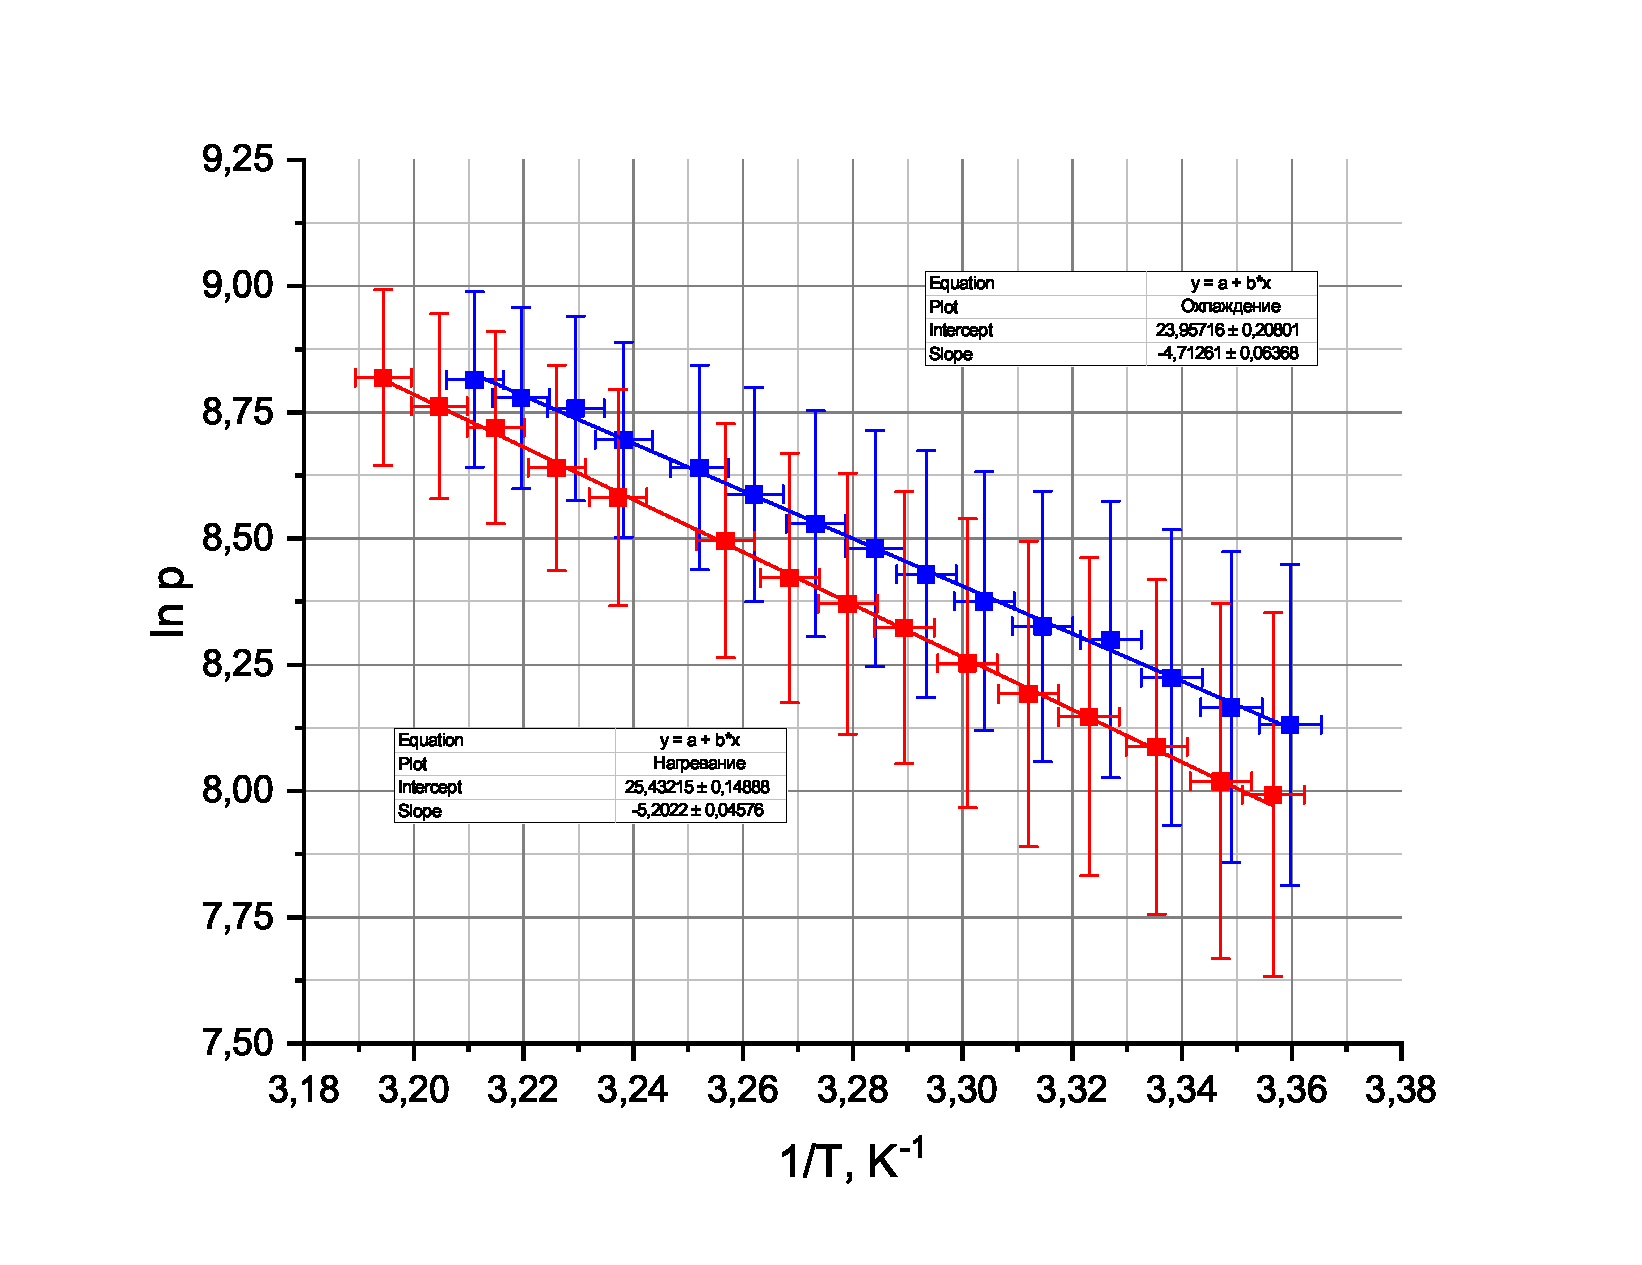
\includegraphics[width=1\linewidth]{4} 
    \caption{Зависимость мощности, потребляемой нитью лампы, $W$ от
абсолютной температуры $T$}
\label{fig:4}
\end{figure}




Измерим яркостную температуру неоновой лампочки:
\[
    T_\text{Ne} \approx 1593\: \text{К} 
\]






\section{Анализ результатов}
Прологарифмируем закон Стефана-Больцмана \eqref{eq:1}, где четвертую степень
заменим на $n$:
\[
    \ln W = \ln (\epsilon_T \sigma S) + n \ln T
\]

По графику на \fig{fig:4} получим $n$:
\[
    n = 4,05 \pm 0,06
\]

Найдем величину постоянной Стефана-Больцмана по формуле:
\[
    \sigma = \frac{W}{\epsilon_T S T^4}
\]

для каждого $T > 1700\ \text{К}$


\begin{table}[H]
\centering
\begin{tabular}{|c|c|}
\hline
$T,\: \text{К}$      & 
\begin{tabular}{c}
    $\sigma \cdot 10^{-8}$ \\[-7pt]
    $\text{Вт} \cdot \text{м}^{-2} \cdot \text{К} ^{-4}$ 
\end{tabular}  \\ \hline
1817,71 & 5,4688 \\ \hline
1943,75 & 5,1994 \\ \hline
2041,67 & 4,9673 \\ \hline
2144,79 & 4,9726 \\ \hline
2246,88 & 4,6075 \\ \hline
2296,88 & 4,4966 \\ \hline
\end{tabular}
\caption{Постоянная Стефана-Больцмана $\sigma$ при температуре $T$}
\end{table}

Усредняя получим:
\[
    \sigma = (4,95 \pm 0,13) \cdot 10 ^{-8}\: \text{Вт} \cdot \text{м}
    ^{-2} \cdot \text{К} ^{-4}
\]

Посчитаем постоянную Планка $h$ по формуле:
\[
    h = 2 \pi \sqrt[3]{ \frac{\pi^2 k^4}{60 c^2 \sigma} }
\]

Получим:
\[
    h = (6,93 \pm 0,06) \cdot 10 ^{-34}\: \text{Дж} \cdot \text{с}
\]









\section{Выводы}
В работе была проведена проверка закона Стефана-Больцмана
\eqref{eq:1}. По графику зависимости мощности, потребляемой нитью
лампы, $W$ от термодинамической температуры $T$ \ffig{fig:4} экспериментально была
определена степень, в которую возводится $T$ в законе
Стефана-Больцмана:
\[
    n = 4,05\pm 0,06
\]
Значение в пределах погрешности совпадает с 4, что подтверждает
возможность использования модели АЧТ и коэффициента серости.

Вычислено значение постоянной Стефана-Больцмана и постоянной Планка по
результатам эксперимента:
\begin{equation*}
    \begin{gathered}
        \sigma = (4,95 \pm 0,13) \cdot 10 ^{-8}\: \text{Вт} \cdot \text{м}
        ^{-2} \cdot \text{К} ^{-4}\\
        h = (6,93 \pm 0,06) \cdot 10 ^{-34}\: \text{Дж} \cdot \text{с}
    \end{gathered}
\end{equation*}

Значения несколько отличаются от табличных:
\begin{equation*}
    \begin{gathered}
        \sigma_\text{т} = 5,6696 \cdot 10 ^{-8}\: \text{Вт} \cdot \text{м}
        ^{-2} \cdot \text{К} ^{-4}\\
        h_\text{т} = 6,6254 \cdot 10 ^{-34}\: \text{Дж} \cdot \text{с}
    \end{gathered}
\end{equation*}

Это связано с селективностью излучения вольфрама (особенно при ярком
накале) и с вычислениями по формулам, которую учитывают какую-то заданную окружающую
температуру \ffig{fig:2}, а не фактическую комнатную при проведении
эксперимента.

Были проведены наблюдения, доказывающую разницу между яркостной
температурой и абсолютной термодинамической температурой. Кольца из
разного материала при одинаковой температуре изменяли свой цвет по
разному, также неоновая лампочка выдавала яркостную температуру сильно
больше ее фактической термодинамической температуры. Это связано с
тем, что яркостная температура по сути характеризует интенсивность
излучения при этом никак не учитывает процессов из-за которых тело
начинает излучать.    









\end{document}
